\glsentryfull{qmla} is an algorithm that extends the concept of applying machine learning to the 
    characterisation of Hamiltonians we've seen so far. 
The extension, and central question of \gls{qmla} is:
    if we do not even have the structure of the model which describes a target quantum system, 
    can we still learn about the physics of the system?
That is, we remove the assumption about the form of the Hamiltonian model, 
    and attempt to uncover which \emph{\glspl{term}} constitute the Hamiltonian, 
    and in so doing, learn what interactions the system is subject to. 
Throughout this thesis, we are concerned solely with Hamiltonian models. 
    although, in general, the description of a quantum system of interest need not be Hamiltonian, 
    e.g. it could be Lindbladian for open quantum systems, 
    so we generalise the effort to the search for the most suitable \emph{\gls{model}}. 
\par 

For the remainder of this thesis, our objective is to learn the model underlying 
    some target system \gls{q}. 
We will first introduce some concepts which will prove useful when discussing \gls{qmla}, 
    before describing the protocol in detail in \cref{sec:qmla_protocol}.


% %%%%%%%%%%% MODELS %%%%%%%%%%% 
\section{Models}\label{sec:models}
\Glspl{model} are simply the mathematical objects which can be used to predict the behaviour of a system. 
In this thesis, \glspl{model} are synonymous with Hamiltonians,
    composed of a set of \emph{\glspl{term}}, $\termset = \{ \hat{t} \}$, 
    where each $\hat{t}$ is a matrix. 
Each term is assosiated with a multipicative scalar, which may be referred to as that term's \emph{parameter}: 
    we impose order on the terms and parameters such that we can succinctly summarise any model as 

\begin{align}
    \label{eqn:model}
    \begin{split}
        \hat{H} = \irow{\alpha_0 & \dots & \alpha_n} \icol{\hat{t}_1 \\ \vdots \\ \hat{t}_n} = \al \cdot \terms 
    \end{split}
\end{align}
    where $\al, \terms$ are the model's parameters and terms, respectively.

For example, a model which is the sum of the (non-identity) Pauli operators is given by
\begin{align}
    \label{eqn:pauli_sum_model}
    \begin{split}
        \hat{H} &= \irow{\alpha_x & \alpha_y & \alpha_z} \cdot \icol{\sx \\ \sy \\ \sz} \\
        &= \alpha_x \sx + \alpha_y \sy + \alpha_z \sz \\
        &= \begin{pmatrix}
            \alpha_z & \alpha_x - i \alpha_y \\
            \alpha_x + i\alpha_y & \alpha_z
        \end{pmatrix}.
    \end{split}
\end{align}
\par 

Through this formalism, we can say that the sole task of \gls{qhl} was to optimise $\al$, given $\terms$. 
The principle task of \gls{qmla} is to identify $\terms$ with the most statistical evidence 
    for describing the target system \gls{q}. 
In short, \gls{qmla} proposes candidate models $\hi$ as hypoteses to explain \gls{q}; 
    we \emph{train} each model independently through a parameter learning routine, 
    and finally nominate the model with the best performance after training. 
In particular, \gls{qmla} uses \gls{qhl} as the parameter learning subroutine, 
    but in principle this step can be performed by any algorithm which learns $\al$ for given $\terms$, 
    \cite{wang2015hamiltonian, krastanov2019stochastic, flurin2020using, niu2019learning, 
    greplova2017quantum,lokhov2018optimal, acampora2019evolutionary, burgarth2017evolution}. 
While discussing a model $\hi$, their \emph{training} then simply means the implementation 
    of \gls{qhl}, where $\hi$ is assumed to represent \gls{q}, 
    such that $\al_i$ is optimised as well as it can be, even if $\hi$ is entirely inaccurate. 

% %%%%%%%%%%% BAYES FACTORS %%%%%%%%%%% 
\section{Bayes factors}\label{sec:bayes_factors}
We can use the tools introduced in \cref{sec:total_log_total_likelihood} to \emph{compare} models. 
Of course it is first necessary to ensure that each model has  
    been adequately trained: while inaccurate models are unlikely to strongly 
    capture the system dynamics, they should first train on the system 
    to determine their best attempt at doing so, 
    i.e. they should undergo the process in \cref{chapter:qhl}.
It is statistically meaningful to compare models via their \gls{tltl}, $\tll_i$, 
    if and only if they have considered the same data, 
    i.e. if models have each attempted to account for the same set of experiments, $\expset$ \cite{kass1995bayes}.
\par 

We can then exploit direct pairwise comparisons between models,  
    by imposing that both models' \gls{tltl} are computed based 
    on \emph{any} shared set of experiments $\expset$, 
    with corresponding measurements $\expdata = \{ d_{e}\}_{e \in \expset}$.
Pairwise comparisons can then be quantified by the \gls{bf},
\begin{equation}
    \label{eqn:bayes_factors}
    B_{ij} = \frac{\Pr(\expdata | \hi; \expset)}{\Pr(\expdata | \hj; \expset)}.
\end{equation}
Intuitively, we see that the \gls{bf} is the ratio of the likelihood, i.e. the performance, 
    of model $\hi$'s attempt to account for the data set $\expdata$ observed following the 
    experiment set $\expset$, against the same \gls{likelihood} for model $\hj$.
\glspl{bf} are known to be statistically signicative of the stronger model 
    from a pair, at explaining observed data,
    while favouring models of low cardinality, thereby supressing overfitting models. 
\par 

We have that, for independent experiments, and recalling \cref{eqn:total_likelihood}, 
\begin{align}
    \begin{split}
        \Pr(\expdata | \hi; \expset) &= \Pr(d_n | \hi; e_n) \times \Pr(d_{n-1} | \hi; e_{n-1}) \times \dots \times \Pr(d_0 | \hi; e_0) \\
        &= \prod_{e \in \expset} \Pr(d_e | \hi; e) \\
        &= \prod_{e \in \expset} (\lk_{e})_i.
    \end{split}
\end{align}

We also have, from \cref{eqn:log_total_likelihood}
\begin{align}
    \label{eqn:log_likelihood}
    \begin{split}
        \tll_{i} &= \sum_{e \in \expset} ln\bk{\bk{\lk_{e}}_i} \\
        \implies e^{\tll_{i}} &= \exp \bk{ \sum_{e \in \expset} ln \left[ \bk{\lk_{e}}_i\right] } 
        = \prod_{e \in \expset} \exp \bk{ ln \left[ (\lk_{e})_i \right]  } 
        = \prod_{e \in \expset} (\lk_{e})_i.
    \end{split}
\end{align}

So we can write 
\begin{align}
    \label{eqn:bf_by_ll}
    \begin{split}
        \bij &= \frac{\Pr(\expdata | \hi; \expset)}{\Pr(\expdata | \hj; \expset)} 
        = \frac{ \prod\limits_{e \in \expset} (\lk_{e})_i } {\prod\limits_{e \in \expset} (\lk_{e})_j } 
        = \frac{e^{\tll_{i}}}{e^{\tll_{j}}} \\
    \end{split}
\end{align}

\begin{equation}
    \label{eqn:bf_succinct}
    \implies \bij = e^{\tll_{i} - \tll_{j}}    
\end{equation}


This is simply the exponential of the difference between two models' total log-likelihoods when presented the same set of experiments. 
Intuitively, if $\hi$ performs well, and therefore has a high \gls{tltl}, $\tll_{i}=-10$, 
    and $\hj$ performs worse with $\tll_{j}=-100$, then $B_{ij} = e^{-10-(-100)} = e^{90} \gg 1$.
Conversely for $\tll_{i}=-100, \tll_{j}=-10$, then $B_{ij} = e^{-90} \ll 1$. 
Therfore $\left| B_{ij} \right|$ is the strength of the statistical evidence
    in favour of the interpretation 

\begin{equation}
    \label{eqn:bf_cases}
    \begin{cases}
        B_{ij} > 1 & \Rightarrow \hi \text{\ stronger than \ } \hj \\
        B_{ij} < 1 & \Rightarrow \hj \text{\ stronger than \ } \hi \\
        B_{ij} = 1 & \Rightarrow \hi \text{\ as strong as \ } \hj \\
    \end{cases}
\end{equation} 

\subsection{Experiment sets}\label{sec:experiments_for_bf}
As mentioned it is necessary for the \gls{tltl} of both models in a \gls{bf} calculation to
    refer to the same set of experiments, $\expset$. 
There are a number of ways to achieve this, 
    which we briefly summarise here for reference later. 
\par 

During training (the \gls{qhl} subroutine), candidate model $\hi$ is trained against $\expset_i$, 
    designed by an \gls{edh} to optimise parameter learning specifically for $\hi$;
    likewise $\hj$ is trained on $\expset_j$. 
The simplest method to compute the \gls{bf} is to enforce $\expset=\expset_i \cup \expset_j$ 
    in \cref{eqn:bayes_factors}, i.e. to cross-train $\hi$ using the data designed specifically for training $\hj$, 
    and vice versa. 
This is a valid approach because it challenges each model to attempt to explain experiments
    designed explicitly for its competitor,   
    at which only truly accurate models are likely to succeed. 
\par 
A second approach builds on the first, but incorporates \emph{burn--in} time in the training regime:
    this is a standard technique in the evaluation of \gls{ml} models whereby its earliest iterations 
    are discounted for evaluation so as not to skew its metrics, 
    ensuring the evaluation reflects the strength of the model. 
In \gls{bf}, we achieve this by basing the \gls{tltl} only on a subset of the training experiments. 
For example, the latter half of experiments designed during the training of $\hi$, $\expset_i^{\prime}$. 
This does not result in less predictive \gls{bf}, since we are merely removing the 
    noisy segments of the training for each model, e.g. the first half of experiments in \cref{fig:param_learning_vary_particles}. 
Moreover it provides a benefit in reducing the computation requirements: 
    updating each model to ensure the \gls{tltl} is based on $\expset^{\prime}=\expset_i^{\prime} \cup \expset_j^{\prime}$
    requires only half the computation time, 
    which can be further reduced by lowering the number of particles used during the update, $\Np^{\prime}$, 
    which will give a similar result as using $\Np$, assuming the posterior has converged.
We will verify this claim later, after we have introduced some relevant concepts, in \cref{sec:bf_by_f_score}. 
\todo{figures to prove these points.}
\par 

A final option is to design a set of \emph{evaluation} experiments, $\expset_v$, 
    that are valid for a broad variety of models, and so will not favour any particular model.
Again, this is a common technique in \gls{ml}: to use one set of data for training models, 
    and a second, unseen dataset for evaluation. 
This is clearly a favourable approach: 
    provided for each model we compute \cref{eqn:log_total_likelihood} using $\expset_v$,
    we can automatically select the strongest model based solely on their \glspl{tltl}, 
    meaning we do not have to perform further computationally-expensive updates, 
    as required to cross-train on opponents' 
    experiments during \gls{bf} calculation. 
However, it does impose on the user to design a \emph{fair} $\expset_v$, 
    requiring unbiased \gls{probe} states $\{\ket{\psi}\}$ and times $\{t\}$ on a timescale 
    which is meaningful to the system under consideration. 
For example, experiments with $t > T_2$, the decoherence time of the system, 
    would result in measurements which offer little information, 
    and hence it would be difficult to extract evidence in favour of any 
    model from experiments in this domain.
It is difficult to know, or even estimate, such meaningful time scales a priori,
    so it is difficult for a user to design $\expset_v$. 
Additionally, the training regime each model undergoes during \gls{qhl}
    is designed to provide adaptive experiments that take into account
    the specific model entertained, to choose an optimal set of evolution times, 
    so it is likely that the set of times in $\expset_i$ is \emph{reasonable} by default. 
This approach would be favoured in principle, in the case where such constraints can be accounted for,
    e.g. an experiment repeated in a laboratory where the available 
    \gls{probe} states are limited and the timescale achievable is understood. 
     
% %%%%%%%%%%% PROTOCOL %%%%%%%%%%%     
\section{Quantum Model Learning Agent Protocol}\label{sec:qmla_protocol}
Given a target quantum system, \gls{q}, described by some \emph{true} model $\ho$, 
    \gls{qmla} distills a model $\hp \approx \ho$.
We can think of \gls{qmla} as a forest search algorithm\footnotemark:
    consisting of a number of trees, each of which can have an arbitrary number of branches, 
    where each leaf on each branch is an individual model, 
    \gls{qmla} is the search for the leaf in the forest with the 
    strongest statistical evidence of representing \gls{q}. 
\footnotetext{
    Note \gls{qmla} is not a random forest, where decision trees are added at random, 
    because in \gls{qmla} trees are highly structured and included manually. 
}    
Each tree in the \gls{qmla} forest corresponds to an independent \emph{ \gls{model search} }, 
    structured according to a bespoke \gls{es}, which we detail in \cref{sec:exploration_strategies}. 
In short, the  \gls{model search}  proceeds by grouping models in \emph{layers},
    training each model on each layer independently,
    layers are then \emph{consolidated} to rank their performance,
    and new models are then \emph{spawned}. 

\begin{figure}[t!]
    \begin{center}
        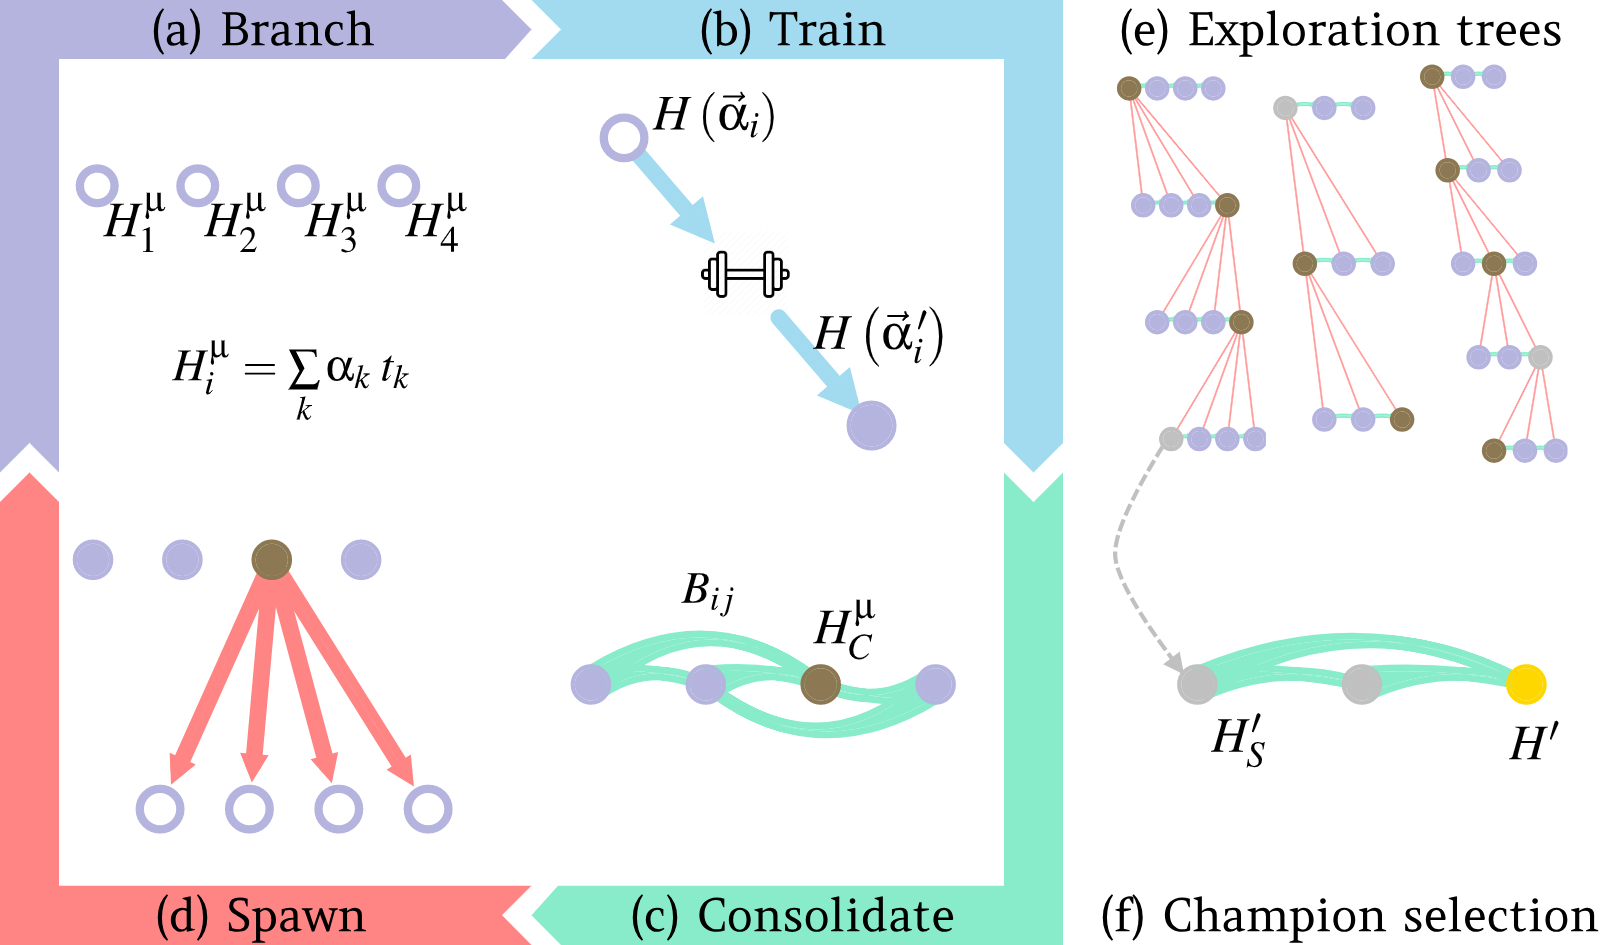
\includegraphics{algorithms/figures/overview.jpg}
    \end{center}
    \caption[Quantum Model Learning Agent overview]{
        Schematic of \acrfull{qmla}. 
        \textbf{(a-d)} \Glsentryfull{model search} phase within an \Glsentryfull{es}.
        \textbf{(a)} Models are placed as (empty, purple) nodes on the \emph{active branch} $\mu$, 
            where each model is a sum of terms $\hat{t}_k$ multiplied by a scalar parameter $\alpha_k$. 
        \textbf{(b)} Each active model is trained according to a subroutine such as 
            quantum Hamiltonian learning to optimise $\al_i$, 
            resulting in the trained $\hat{H}(\al_i^{\prime})$ (filled purple node). 
        \textbf{(c)} $\mu$ is consolidated, i.e. models are evaluated relative to other
            models on $\mu$, according to the consolidation mechanism specificed by the \gls{es}.
            In this example, pairwise Bayes factors $B_{ij}$ between $\hi, \hj$ are computed, 
            resulting in the election of a single branch champion $\hat{H}_C^{\mu}$ (bronze). 
        \textbf{(d)} A new set of models are \emph{spawned} according to the chosen
            \gls{es}'s model genertion strategy.
            In this example, models are spawned from a single parent. 
            The newly spawned models are placed on the next layer $\mu+1$, 
            iterating back to \textbf{(a)}.
        \textbf{(e-f)} Higher level of entire QMLA procedure.
        \textbf{(e)} The  \gls{model search}  phase for a unique \gls{es} is presented on an \emph{exploration tree}. 
            Multiple \gls{es} can operate in parallel, e.g. assuming different underlying physics, 
            so the overall \gls{qmla} procedure involves a \emph{forest search} across multiple exploration trees.
            Each \gls{es} nominates a champion, $\hat{H}_{S}^{\prime}$ (silver), 
            after consolidating its branch champions (bronze). 
        \textbf{(f)} $\hat{H}_{S}^{\prime}$ from each of the above exploration trees are gathered on a single layer, 
            which is consolidated to give the final \gls{champion model}, $\hp$ (gold). 
    }
    \label{fig:qmla_overview}
\end{figure}

% %%%%%%%%%%% EXPLORATION STRATEGIES %%%%%%%%%%% 
\section{Exploration Strategies}\label{sec:exploration_strategies}
\gls{qmla} is implemented by running $\Nt$ \glspl{et} concurrently, 
    where each \gls{et} corresponds to  a unique  \gls{model search}  and ultimately nominates a single 
    model as its favoured approximation of $\ho$. 
An \gls{es} is the set of rules which guide a single \gls{et} throughout its  \gls{model search} . 
We elucidate the responsibilities of \glspl{es} in the remainder of this section, but in short they can be summarised as: 

\begin{easylist}[enumerate]
    \ListProperties(Numbers=r)
    & model generation: 
        combining the knowledge progressively acquired on the \gls{et} to construct new candidate models;
    & decision criteria for the  \gls{model search}  phase:
        instructions for how \gls{qmla} should respond at predefined junctions, 
        e.g. whether to cease the  \gls{model search}  after a branch has completed;
    & \gls{true model} specification:
        detailing the terms and parameters which constitute $\ho$ (in the case where \gls{q} is simulated);
    & modular functionality: 
        subroutines called throughout \gls{qmla} are interchangeable such that each \gls{es} specifies the 
        set of functions to achieve its goals.
\end{easylist}
\par 

\gls{qmla} acts in tandem with one or more \glspl{es}, through the process depicted in \cref{fig:qmla_flow}. 
In summary: 
    \gls{qmla} sends a request to the \gls{es} for a set of models; 
    \gls{es} designs models and places them as leaves on one of its branches, and returns the set $\mathbb{H}$; 
    \gls{qmla} places $\mathbb{H}$ on a unique layer; 
    \gls{qmla} trains the models in $\mathbb{H}$; 
    \gls{qmla} consolidates $\mathbb{H}$;
    \gls{qmla} informs the \gls{es} of the results of training/consolidation of $\mathbb{H}$; 
    \gls{es} decides whether to continue the search, and informs \gls{qmla}.
\tikzstyle{startstop} = [
    rectangle, rounded corners, 
    minimum width=12cm, 
    minimum height=2cm,
    % text top, 
    text centered, 
    text width=7cm, 
    text depth=1mm,
    text height=-5mm,
    draw=black, 
    fill=red!30
]
\tikzstyle{io} = [
    trapezium, trapezium left angle=70, trapezium right angle=110, minimum width=3cm,
    minimum height=1cm, text width = 3cm, text centered, draw=black, fill=blue!30
]
\tikzstyle{process} = [
    rectangle, 
    minimum width=5cm, 
    minimum height=2cm, 
    text centered, 
    text width=4.5cm, 
    text depth=3mm,
    text height=-100mm,
    draw=black, 
    fill=orange!30
]

\tikzstyle{decision} = [
    rectangle,
    % trapezium, 
    % trapezium left angle=70, 
    % trapezium right angle=110, 
    minimum width=2cm, 
    minimum height=1cm, 
    text width = 1.8cm, 
    text centered, 
    draw=black, 
    fill=green!30
]
\tikzstyle{decided} = [
    rectangle, 
    minimum width=0.5cm, 
    minimum height=1cm, 
    text centered, 
    text width=1cm, 
    draw=black, 
    fill=blue!30
]
\tikzstyle{qmla_step} = [
    circle, 
    fill=white, 
    draw=red, 
    text=red, 
    minimum size=0.65cm
]

\tikzstyle{arrow} = [thick,->,>=stealth]



\begin{figure}
    \begin{center}
    
    \begin{tikzpicture}[node distance=2.25cm]
    
    \node (qmla) [startstop, label={[shift={(0ex,-5ex)}]north:Quantum Model Learning Agent}] {};
    
    \node (es) [process, below of=qmla, xshift=-1cm, ] {Exploration Strategy};
    
    \node (qhl) [process, below of=es] {Model Trainer};   

    \node (system) [decision, right of=qhl,  xshift=1cm, below of=qhl] {System \gls{q}};   

    \node (simulator) [decision, below of=system, yshift=0.5cm, ] {Simulator};   

    \node (champion) [decided, below of=simulator, yshift=0.5cm, xshift=-1cm, left of=simulator] {$\hat{H}^{\prime}_{S}$};   
 
    \draw [arrow, red] ([yshift=+0.5cm]es.west) -| node[qmla_step]{1}  ([xshift=-4cm]qmla.south);
    \draw [arrow, red] ([xshift=-4.5cm]qmla.south) |- node[qmla_step]{2a}  ([yshift=-0.5cm]es.west);
    \draw [arrow, red] ([yshift=-10pt]es.east)  -| node[qmla_step]{2c}  ([xshift=+62.5pt]qmla.south);
    \draw [arrow, red] ([xshift=-5.1cm]qmla.south) |- node[qmla_step]{4a}  ([yshift=-10pt]qhl.west);
    \draw [arrow, red] ([xshift=+0.5cm]qhl.south) |- node[qmla_step]{4d}  ([yshift=+0pt]system.west);
    \draw [arrow, red] ([xshift=+1.25cm]qhl.south) |- node[qmla_step]{4e}  ([yshift=+0pt]simulator.west);
    \draw [arrow, red] ([yshift=-10pt]qhl.east) -| node[qmla_step]{4g} ([xshift=+2.75cm]qmla.south) ;
    \draw [arrow, red] ([xshift=+5.5cm]qmla.south) |- node[qmla_step]{7}  ([yshift=+0pt]champion.east);
    
    % \node (step_4) [qmla_step, left of=(0.1cm of qmla), above=(0.1cm of qmla.south)]{4};
    \node (step_3) [qmla_step, left of=qmla.west, xshift=0cm, above=(0.1cm of qmla.south)]{3};
    \node (step_5) [qmla_step, right of=step_3, xshift=3.75cm, ]{5};
    \node (step_6) [qmla_step, right of=step_5, xshift=-1cm,]{6};
    % \node (step_6a) [qmla_step, right of=step_6, xshift=-1cm]{6a};

    \node (step_2b) [qmla_step, above=(0.1cm of es.south)]{2b};

    \node (step_4b) [qmla_step, right of=qhl.west, xshift=-4cm, above=(0.1cm of qhl.south)]{4b};
    \node (step_4c) [qmla_step, right of=step_4b, xshift=-1cm]{4c};
    \node (step_4f) [qmla_step, right of=step_4c, ]{4f};


    \end{tikzpicture}
    \end{center}
    
    \caption[Interface between \glsentryshort{qmla} and a single \glsentrylong{es}]{
        Interface between \glsentryfull{qmla} and a single \glsentryfull{es}
        The main components are the \gls{es}, model training subroutine, target quantum system (i.e. black box, \gls{q}), 
        and (quantum) simulator. 
        The main steps of the algorithm, shown in red with arrows denoting data transferred during that step, are as follows.
        \textbf{1}, QMLA retrieves decision infrastructure from ES, such as the consolidation mechanism and termination criteria.
        \textbf{2}, models are designed/spawned; 
        \textbf{2a}, QMLA signals to ES requesting a set of models, passing the results of the previous layers' models if appropriate.
        \textbf{2b}, ES spawns new models, $\mathbb{H}$;
        \textbf{2c}, ES passes $\mathbb{H}$ to QMLA. 
        \textbf{3}, QMLA assigns a new layer $(\mu \gets \mu + 1)$ and places the newly proposed models upon it.
        \textbf{4}, Model training subroutine (here quantum Hamiltonian learning), performed independently for each model $\hi \in \mu$; 
        \textbf{4a}, QMLA passes $\hi$ to the model trainer; 
        \textbf{4b}, construct a prior distribution $P_i$ describing the model's parameterisation $\vec{\alpha}_i$;
        \textbf{4c}, design experiment $e$ to perform on \gls{q} to optimise $\vec{\alpha}_i$;
        \textbf{4d}, perform $e$ on \gls{q} to retrieve a datum $d$;
        \textbf{4e}, simulate $e$ for particles $\{ \vec{\alpha}_1, \dots , \vec{\alpha}_N \}$ 
            sampled from $P_i$ to retrieve a \emph{likelihood} $\lk_{e}$;
        \textbf{4e}, update the prior $P_i$ based on $(d, \lk_{e})$.
        \textbf{5}, Evaluate and rank $\hi \in \mu$ according to the ES's consolidation mechanism.
        \textbf{6}, Check ES's termination criteria; if reached, proceed to \textbf{(7)}, otherwise return to \textbf{(2)}.
        \textbf{7}, Nominate \gls{champion model}, $\hp_{S}$.        
    }
    \label{fig:qmla_flow}
\end{figure}

   

\subsection{Model generation}\label{sec:model_generation}
The main role of any \gls{es} is to design candidate models to test against $\ho$. 
This can be done through any means deemed appropriate, 
    although in general it is sensible to exploit the information gleaned so far in the \gls{et}, 
    such as the performance of previous candidates and their comparisons, 
    so that successfel models are seen to \emph{\gls{spawn}} new models, 
    e.g. by combining previously successful models, or by building upon them. 
Conversely, model generation can be completely determined in advance or entirely random.
This alludes to the central design choice in composing an \gls{es}: 
    how broad and deep should the searchable \emph{model space} be, 
    considering that adequately training each model
    is expensive, and that model comparisons are similarly expensive. 
The  \gls{model search}  occurs within some \emph{\gls{model space}}, the size of which can usually be easily found 
    by assuming that terms are binary -- either the interaction they represent is present or not. 
If all possible terms are accounted for, and the total set of terms is $\termset$,
    then there are $2^{\absval{\termset}}$ available candidates in the model space. 
The \gls{model space} encompasses the closed\footnotemark set of models construable by the set of terms considered by an \gls{es}. 
Because training models is slow in general,
    a central aim of \gls{qmla} is to search this space efficiently,
    i.e. to minimise the number of models considered, while retaining high quality models and 
    providing a reasonable prospect of uncovering the  \gls{true model} , or a strong approximation thereof. 

\footnotetext{
    It is feasible to define an \gls{es} which uses an open model space, that is, there is no pre-defined $\termset$, 
    but rather the \gls{es} determines models through some other heuristic mechanism. 
    In this thesis, we do not propose any such \gls{es}, but note that the \gls{qmla} framework 
    facilitates the concept, see \cref{chapter:sw}.   
}



\subsection{Decision criteria for the model search phase}
Further control parameters, which direct the growth of the \gls{et}, are set within the \gls{es}.
At several junctions within Algs. \cref{alg:qmla}, \cref{alg:model_search}, 
    \gls{qmla} queries the \gls{es} in order to decide what happens next.
Here we list the important cases of this behaviour. 

\begin{description}

    \item[Parameter-learning settings] \
    
    \begin{easylist}[itemize]
    && such as the prior distribution to assign each parameter during \gls{qhl}, and the parameters needed to run \gls{smc}.
    && the time scale on which to examine \gls{q}.
    && the input probes to train upon. 
    \end{easylist}
    
    \item[Branch comparison strategy] \
    \begin{easylist}
    && How to compare models within a branch (or \gls{qmla} layer). Some examples used in this work are
        &&& a points-ranking where each points are assigned according to Eqn. \cref{eqn:bf_cases};
        &&& ranking reflecting each model's log-likelihood after training;
        &&& models are ranked according to some \glsentrylong{of}.
    \end{easylist}

    \item[\gls{model search} termination criteria] \
    \begin{easylist}    
    && e.g. instruction to stop after a fixed number of iterations, or when a certain fitness has been reached.        
    \end{easylist}
    
    \item[Champion nomination] \
    \begin{easylist}    
    && when a single tree is explored, identify a single champion from the branch champions
    && if multiple trees are explored, how to compare champions across trees. 
    \end{easylist}
\end{description}

\subsection{True model specification}
It is necessary also to specify details about the \gls{true model} $\ho$, 
    at least in the case where \gls{qmla} acts on simulated data. 
Within the \gls{es}, we can set $\terms_0$ as well as $\al_0$. 
For example where the target system is an untrusted quantum simulator to be characterised, 
    $S_u$, by interfacing with a trusted (quantum) simulator $S_t$, 
    we decide some $\ho$ in advance:
    the model training subroutine calls for  \glspl{likelihood}, 
    those corresponding to $\ho$ are computed $S_u$, 
    while particles'  \gls{likelihood} are computed on $S_t$. 

\subsection{Modular functionality}\label{sec:modular_functionality}
Finally, there are a number of fundamenetal subroutines which are called upon throughout the \gls{qmla} algorithm. 
These are written independently such that each subroutine has a number of available implementations. 
These can be chosen to match the requirements of the user, and are set via the \gls{es}. 

\begin{description}
    \item[Model training procedure] \
    \begin{easylist}
        && i.e. whether to use \gls{qhl} or quantum process tomography, etc. 
        && In this work we always used \gls{qhl}.     
    \end{easylist}

    \item[ \gls{likelihood} function] the method used to estimate the \gls{likelihood} 
        for use during \gls{qle} within \gls{qhl}, 
        which ultimately depends on the measurement scheme. 
    \begin{easylist}
        && By default, here we use projective measurement back onto the input \gls{probe} state, 
            $\left| \bra{\psi} e^{-i\hat{H}t} \ket{\psi} \right|^2$.        
        && The role of these functions is to compute $\Pr(0)$ to be used by QInfer, 
            which is not always the same as computing the likelihood,
            although these are equiavelent when we measure $d=0$, see .
        &&& Generically, without referring to the likelihood, these functions are to compute the expectation value
                of the unitary operator corresponding to the model of the system.        
        && It is possible to change this to implement any measurement procedure, 
            for example an experimental procedure where the environment is traced out.
    \end{easylist}
            
    \item[\gls{probe}] defining the input probes to be used during training. 
    \begin{easylist}   
        && In general it is preferable to use numerous probes in order to avoid biasing particular terms. 
        && In some cases we are restricted to a small number available input probes, e.g. to match experimental constraints.
    \end{easylist}

    \item[Experiment design heuristic] bespoke experiments to maximise the information 
        on which models are individually trained.
    \begin{easylist}
        && In particular, in this work the experimental controls consist solely of $\{ \ket{\psi}, t \}$. 
        && Currently, probes are generated once according to the previous point, 
            but in principle it is feasible to choose optimal probes based on available or hypothetical information. 
            For example, probes can be chosen as a normalised sum of the candidate model's eigenvectors.
        && Choice of $t$ has a large effect on how well the model can train. 
            By default times are chosen proportional to the inverse of the 
            current uncertainty in $\al$ to maximise Fischer information, 
            through the multi-particle guess heuristic \cite{Wiebe:2014qhl}.
            Alternatively, times may be chosen from a fixed set to force \gls{qhl} to 
            reproduce the dynamics within those times' scale. 
            For instance, if a small amount of experimental data is available offline, 
            it is sensible to train all candidate models against the entire dataset.  
    \end{easylist}

    \item[Model training prior] change the prior distribution, e.g. Fig. \cref{fig:qhl_smc}(a)

\end{description}

\subsection{Exploration strategy examples}
To solidifiy the concept of \glspl{es}, and how they affect the overall,
    reach and runtime of a given \gls{et}, consider the following examples, 
    where each strategy specifies how models are generated, as well as how trained models are compared within a branch. 
Recall that all of these strategies rely on \gls{qhl} as the model training strategy, 
    so that the run time for training, is $t_{\textrm{QHL} \sim \Ne\Np t_U}$, 
    where $t_U(n)$ is the time to compute the unitary evolution via the matrix exponential for an $n$-qubit model 
All models are trained using the default  \gls{likelihood} in \cref{eqn:likelihood}. 
Assume the conditions
\begin{easylist}[itemize]
    & all models considered are represented by 4-qubit models;
    && $t_{U(4)} \sim 10^{-3}\textrm{sec}$. 
    & each model undergoes a reasonable training regime;
    && $\Ne=1000, \Np=3000$;
    && $\implies t_{\textrm{QHL}} = \Ne \times \Np \times  t_{U(4)} = 3000s \sim 1 \textrm{h} $;
    & Bayes factor calculations use 
    && $\Ne=500, \Np=3000 $
    && $\implies t_{\textrm{BF}} \sim 2 \times  500 \times 3000 \times  10^{-3} \sim 1 \textrm{h}$;
    & there are 12 available terms
    && allowing any combination of terms, this admits a \gls{model space} of size $2^{12} = 4096$
    & access to 16 computer cores to parallelise calculations over
    && i.e. we can train 16 models or perform 16 \gls{bf} comparisons in $1h$.
\end{easylist}
\par 

\noindent Then, consider the following model generation/comparison strategies.
\begin{easylist}[enumerate]
    \ListProperties(Numbers1=l, Numbers2=r)
    & \label{gr:predefined} Predefined set of $16$ models, comparing every pair of models
    && Training takes $1h$, and ${16 \choose 2} = 120$ comparisons need $8h$
    && total time is $9h$. 
    & \label{gr:generative_full} Generative procedure for model design, comparing every pair of models,
        running for 12 branches
    && One branch takes $9h \implies$ total time is $12 \times 9 = 108h$; 
    && total number of models considered is $16 \times 12 = 192$. 
    & \label{gr:generative_sparse} Generative procedure for model design, where less model comparisons are needed 
        (say one third of all model pairs are compared),
        running for 12 branches
    && Training time is still $1h$
    && One third of comparisons, i.e. $40$ \gls{bf} to compute, requires $3h$
    && One branch takes $4 h \implies$ total time is $36 h$
    && total number of models considered is also $192$. 
\end{easylist}

These examples illustrate some of the design decisions involved in \gls{es}s, 
    namely whether timing considerations are more important than thoroughly exploring the model space.
They also show considerable time--savings in cases where it is
    acceptable to forego all model comparisons. 
The approch in \cref{gr:predefined} is clearly limited in its applicability, 
    mainly in that there is a heavy requirement for prior knowledge, 
    and it is only useful in cases where we either know $\ho \in \mathbb{H}$, 
    or would be satisfied with approximating $\ho$ as the closest available $\hj \in \mathbb{H}$. 
On the opposite end of this spectrum, \cref{gr:generative_sparse}  is an excellent approach
    with respect to minimising prior knowledge required by the algorithm, 
    although at the significant expense of testing a much larger number of candidate models. 
There is no optimal strategy for all use--cases: 
    specific quantum systems of study demand particular considerations, 
    and the amount of prior information available informs how wide the model search should reach. 

\par 

In this work we have used two straightforward model generation routines.
Firstly, during the study of various physical classes (Ising, Heisenberg, Fermi-Hubbard), 
    a list of lattice configurations were chosen in advance,
    which were then mapped to Hamiltonian models.
This \gls{es} is non-adaptive and indeed the model search
    consists merely of a single branch with no subsequent calls to the model generation routine, 
    as in \cref{gr:predefined}. 
In the latter section instead we use a \gls{ga}:
    this is clearly a far more general strategy, at a significant computational cost, 
    but is suitable for systems where we have less knowledge in advance. 
In this case, new models are designed based heavily on results from earlier branches of the \gls{et}. 
The genetic algorithm model generation subroutine is listed in \cref{alg:generate_models}, 
    and can broadly be summed up thus: 
    the best models in a generation $\mu$ produce offspring which constitute models on the next generation.
These types of evolutionary algorithms ensure that newly proposed candidates inherit 
    some of the structure which rendered previous candidates (relatively) successful, 
    in the expectation that this will yield ever-stronger candidates. 

% %%%%%%%%%%% GENERALITY %%%%%%%%%%% 

\section{Generality}
Several aspects of \gls{qmla} are deliberately vague in order to facilitate generality. 

\begin{description}
    \item[\Gls{model}] can mean any description of a quantum system which captures the interactions it is subject to. 
    \begin{easylist}[itemize]
        && Here we exclusively consider Hamiltonian models, but Lindbladian models can also be considered as generators of quantum dynamics. 
    \end{easylist}
    \item[Model training] is any subroutine which can train a given model, i.e. optimise a given parameterisation 
        under the assumption that represents the target system. 
    \begin{easylist}[itemize]
        && Currently only \gls{qhl} has been used, but tomography is valid in principle, albeit slower. 
        && \Gls{qhl} relies on the calculation of a characteristic  \gls{likelihood} function; 
            this too is not restricted to the generic form of \cref{eqn:likelihood} and can be replaced by 
            any form which represents the \gls{likelihood} that experimental conditions $e$ result in measurement datum $d$. 
            We will see examples of this in \cref{chapter:nv} where we trace out part of the system in order 
            to represent open systems. 
    \end{easylist}
    \item[Model selection] or \emph{consolidation} can be as rigourous as desired by the user. 
    \begin{easylist}[itemize]
    && Consolidation occurs at the branch level of each \gls{et}, but also in finding the tree champion, 
        and ultimately the global champion. 
    && In practice, we use either \gls{bf} or a related concept such as \gls{tltl} which are statistically signicative. 
        However, in \cref{chapter:ga} we will consider a number of alternative schemes for discerning the strongest models. 
    \end{easylist}
\end{description}

\subsection{Agency}\label{sec:agency}
While the concept of \emph{agency} is contentious \cite{franklin1996agent}, 
    we can view our overall protocol as a multi-agent system \cite{wooldridge2009introduction}, 
    or even an agent based evolutionary algorithm \cite{sarker2010agent}, 
    because any given \gls{es} satisfies the definition,
    \emph{the  population  of  individuals can be considered as a population of agents}, 
    where we mean the population of models present on a given \gls{et}. 
More precisely, we can view individual models as \emph{learning agents} according to the criteria of 
    \cite{russell2002artificial}, i.e. that a learning agent has
    \begin{easylist}[itemize]
        & a \emph{problem generator}: designs actions in an attempt to learn about the system -- this is precisely the role of the \gls{edh};
        & a \emph{performance element}: implements the the designed actions and measures the outcome
            -- the measurement of a datum following the experiment chosen by the \gls{edh}; 
        & a \emph{critic}: the likleihood function informs whether the designed action (experiment) was successful; 
        & a \emph{learning element}: the updates to the weights and overall parameter distribution improve the model's performance over time. 
    \end{easylist}
We depict this analogy in \cref{fig:learning_agent}.
Finally, the model design strategy encoded in the \gls{es} \emph{can} allow agency,
    by permitting the spawn rules autonomy, 
    so we label the entire procedure as the quantum model learning agent. 

\tikzstyle{startstop} = [
    rectangle, rounded corners, 
    minimum width=12cm, 
    minimum height=2cm,
    % text top, 
    text centered, 
    text width=7cm, 
    text depth=1mm,
    text height=-5mm,
    draw=black, 
    fill=red!30
]
\tikzstyle{io} = [
    trapezium, trapezium left angle=70, trapezium right angle=110, minimum width=3cm,
    minimum height=1cm, text width = 3cm, text centered, draw=black, fill=blue!30
]

\tikzstyle{environment} = [
    rectangle, rounded corners, 
    minimum width=3cm, 
    minimum height=8.5cm,
    % text top, 
    text centered, 
    % text width=1.5cm, 
    % text depth=1mm,
    % text height=-5mm,
    draw=black, 
    fill=red!30
]
\tikzstyle{process} = [
    rectangle, 
    minimum width=3cm, 
    minimum height=1.5cm, 
    text centered, 
    text width=2cm, 
    draw=black, 
    fill=orange!30
]

\tikzstyle{decision} = [
    rectangle,
    % trapezium, 
    % trapezium left angle=70, 
    % trapezium right angle=110, 
    minimum width=2cm, 
    minimum height=1cm, 
    text width = 1.8cm, 
    text centered, 
    draw=black, 
    fill=green!30
]
\tikzstyle{decided} = [
    rectangle, 
    minimum width=0.5cm, 
    minimum height=1cm, 
    text centered, 
    text width=1cm, 
    draw=black, 
    fill=blue!30
]
\tikzstyle{agent_step} = [
    circle, 
    % fill=white, 
    % draw=red, 
    text=red, 
    minimum size=0.65cm
]

\tikzstyle{arrow} = [thick,->,>=stealth]


\usetikzlibrary{calc}
\tikzset{>=latex}
\tikzstyle{a}=[fill=red,circle,inner sep=2pt]
\tikzstyle{b}=[fill=blue,circle,inner sep=2pt]

% \begin{tikzpicture}
%   \node [a] (A) at (0,0) {};
%   \node [b] (B) at (4,0.8) {};

%   \coordinate (A2) at ($ (A) - (0,1) $);
%   \coordinate (B2) at ($ (B) - (0,1) $);
%   \coordinate (B3) at ($ (B)!(A2)!(B2) $);

%   \draw [<->,very thick] (A2) -- (B3);
% \end{tikzpicture}


\begin{figure}
    \centering
    \begin{minipage}[c]{0.4\textwidth}
    
        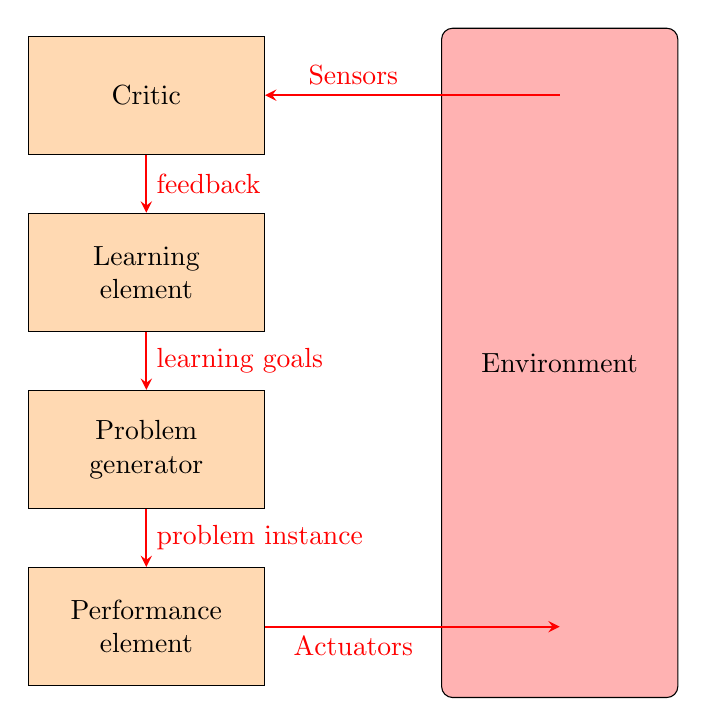
\begin{tikzpicture}[node distance=2.25cm]
        
        \node (critic) [ process] {Critic};
        \node (learning_element) [process, below of=critic] {Learning element};   
        \node (problem_generator) [process, below of=learning_element,] {Problem generator};   
        \node (performance_element) [process, below of=problem_generator,] {Performance element};   
        \node (environment) [environment, right of=critic, xshift=3cm, yshift=-3.4cm] {Environment};   
    
        \coordinate (B1) at ($ (environment) + (0,1)$);
        \coordinate (B2) at ($ (environment) - (0,1)$);
        \coordinate (perf_env) at ($ (environment)!(performance_element.east)!(B2) $);
        \coordinate (env_critic) at ($ (environment)!(critic.east)!(B1) $);

        \draw [arrow, red] (critic.south) -- node[anchor=west]{feedback} (learning_element.north);
        \draw [arrow, red] (learning_element.south) -- node[anchor=west, ]{learning goals} (problem_generator.north);
        \draw [arrow, red] (problem_generator.south) -- node[anchor=west, ]{problem instance} (performance_element.north);
        \draw [arrow, red] (performance_element.east) -- node[anchor=north, xshift=-0.75cm]{Actuators} (perf_env);
        \draw [arrow, red] (env_critic) -- node[anchor=south,xshift=-0.75cm]{Sensors} (critic.east);
        
        \end{tikzpicture}
    \end{minipage}
    ~\hspace{2cm}
    \begin{minipage}[c]{0.4\textwidth}
    
        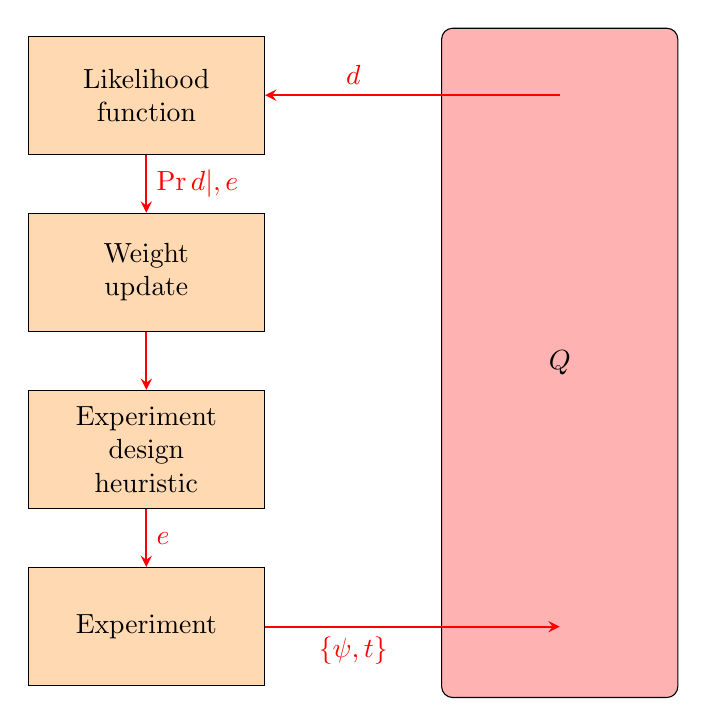
\begin{tikzpicture}[node distance=2.25cm]
        
        \node (critic) [ process] {Likelihood function};
        \node (learning_element) [process, below of=critic] {Weight update};   
        \node (problem_generator) [process, below of=learning_element,] {Experiment design heuristic};   
        \node (performance_element) [process, below of=problem_generator,] {Experiment};   
        \node (environment) [environment, right of=critic, xshift=3cm, yshift=-3.4cm] {$Q$ };   
    
        \coordinate (B1) at ($ (environment) + (0,1)$);
        \coordinate (B2) at ($ (environment) - (0,1)$);
        \coordinate (perf_env) at ($ (environment)!(performance_element.east)!(B2) $);
        \coordinate (env_critic) at ($ (environment)!(critic.east)!(B1) $);

        \draw [arrow, red] (critic.south) -- node[anchor=west]{$\Pr\bk{d | \al, e}$} (learning_element.north);
        \draw [arrow, red] (learning_element.south) -- node[anchor=west, ]{$\pra$} (problem_generator.north);
        \draw [arrow, red] (problem_generator.south) -- node[anchor=west, ]{$e$} (performance_element.north);
        \draw [arrow, red] (performance_element.east) -- node[anchor=north, xshift=-0.75cm]{$\{ \ket{\psi}, t \}$} (perf_env);
        \draw [arrow, red] (env_critic) -- node[anchor=south,xshift=-0.75cm]{$d$} (critic.east);
        
        \end{tikzpicture}
    \end{minipage}


    \caption[Learning agents]{
        Learning agents. \textbf{Left}: definition of a learning agent, where an \emph{environment} is affected by 
        \emph{actuators} which realise a \emph{problem instance}, designed by a \emph{problem generator}, through some \emph{performance element}. 
        The result of the agent's action is detected by \emph{sensors}, which the \emph{critic} interprets with respect to
        the agent's \emph{learning goals}, by providing \emph{feedback} to the \emph{learning element}. 
        \emph{Right}: mapping of the concept of a learning agent on to an individual model. 
        A target quantum system, $Q$, is queried by performing some experiment $e$, 
        designed by an experiment design heuristic, and implemented by evolving a probe state $\ket{\psi}$ for time $t$. 
        The systems is measured, and the datum $d$ is sent to the \gls{likelihood} function, which sends the likelihood $\Pr(d|\al, t)$
        to the weight update (and the parameter distribution update), before designing another experiment. 
    }
    \label{fig:learning_agent}
\end{figure}

   


%%%%%%%%%%% PSEUDOCODE %%%%%%%%%%% 
\section{Algorithms}
We conclude this chapter by listing the algorithms used most frequently, 
    in order to clarify each of their roles, and how they interact. 
\cref{alg:qmla} shows the overall \gls{qmla} algorithm, 
    which is simplified greatly to a loop over the  \gls{model search}  of each \gls{es}. 
The  \gls{model search}  iteself is listed in \cref{alg:model_search},
    which contains calls to subroutines for model learning (\gls{qhl}, \cref{alg:qhl}), 
    branch evaluation (which can be based upon \gls{bf}, \cref{alg:bayes_factor})
    and centers on the generation of new models, an example of which -- based on a genetic algorithm -- 
    is given in  \cref{alg:generate_models}. 

\begin{algorithm}
    \caption{Quantum Model Learning Agent}
    \label{alg:qmla}
    \DontPrintSemicolon
    \KwIn{ $Q$ \tcp*[1]{some physically measurable or simulateable quantum system}}
    \KwIn{ $\mathbb{S}$ \tcp*[1]{set of exploration strategies}}\;

    \KwOut{$\hat{H}^{\prime}$ \tcp*[1]{\gls{champion model}}}\;
    
    $\mathbb{H}_c \gets \{\}$\;   
    \For{$S \in \mathbb{S}$ }{
        $\hat{H}_{S}^{\prime} \gets$ \ttt{model\_search(Q, S)} 

        $\mathbb{H}_c \gets \mathbb{H}_c \cup  \{\hat{H}_{S}^{\prime}\}$ \tcp*[1]{add ES champion to collection}
    }
    $\hat{H}^{\prime} \gets $ \ttt{final\_champion($\mathbb{H}_c$)}\;
    return $\hat{H}^{\prime}$

\end{algorithm}

\begin{algorithm}
    \caption{ES subroutine: \ttt{model\_search}}
    \label{alg:model_search}
    \DontPrintSemicolon
    \KwIn{ $Q$ \tcp*[1]{some physically measurable or simulateable quantum system}}
    \KwIn{ $S$ \tcp*[1]{Exploration strategy: collection of rules/subroutines}}\;

    \KwOut{$\hat{H}_{S}^{\prime}$ \tcp*[1]{Exploration strategy's nominated \gls{champion model}}}\;
     
    $\nu \gets \{\}$

    $\mathbb{H}_c \gets \{\}$\;   
    \While{ \ttt{!S.terminate()} }{
        $\mu \gets $ \ttt{S.generate\_models($\nu$)} \tcp*[1]{e.g. \cref{alg:generate_models}}\; 

        \For{ $\hi \in \mu$}{
            $\hi^{\prime} \gets $ \ttt{S.train($\hi$)} \tcp*[1]{e.g. \cref{alg:qhl}}
        }
        $\nu \gets$ \ttt{S.evaluate($\mu$)} \tcp*[1]{e.g. pairwise via \cref{alg:bayes_factor}}

        $\hat{H}_{c}^{\mu} \gets $ \ttt{S.branch\_champion($\nu$)} \tcp*[1]{use $\nu$ to select a branch champion}

        $\mathbb{H}_c \gets \mathbb{H}_c \cup \{\hat{H}_c^{\mu}\}$ \tcp*[1]{add branch champion to collection}
    }

    $\hat{H}_{S}^{\prime} \gets $ \ttt{S.nominate\_champion($\mathbb{H}_c$)}\;
    return $\hat{H}_{S}^{\prime}$

\end{algorithm}


\begin{algorithm}
    \caption{ES subroutine: \ttt{generate\_models} (example: greedy spawn)}
    \label{alg:generate_models}
    \DontPrintSemicolon
    \KwIn{ $\nu$ \tcp*[1]{information about models considered to date}}\;

    % TODO 
    return $\mathbb{H}$ 

\end{algorithm}



\begin{algorithm}
    \caption{Quantum Hamiltonian Learning}
    \label{alg:qhl}
    \DontPrintSemicolon
    \KwIn{ $Q$ \tcp*[1]{some physically measurable or simulatable quantum system, described by $\ho$}}

    \KwIn{$\hat{H}_i$ \tcp*[1]{Hamiltonian model attempting to reproduce data from $\hat{H}_0$ }}
    \KwIn{$\pra$ \tcp*[1]{probability distribution for $\al = \al_0 $}}
    \KwIn{$\Ne$ \tcp*[1]{number of epochs to iterate learning procedure for}}
    \KwIn{$\Np$ \tcp*[1]{number of particles to draw from $\pra$}}
    \KwIn{\ttt{$\Lambda(\pra)$} \tcp*[1]{Heuristic algorithm which designs experiments}}
    \KwIn{\ttt{RS($\pra$)} \tcp*[1]{Resampling algorithm for redrawing particles}}

    \KwOut{$\al^{\prime}$ \tcp*[1]{estimate of Hamiltonian parameters}}\;


    Sample $\Np$ times from $\pra \gets \mathcal{P}$ \tcp*[1]{particles}\;
    
    \For{$ e \in  \{1 \rightarrow \Ne\}$ }{ 
        
        $t, \ket{\psi} \gets \Lambda(\pra)$ \tcp*[1]{design an experiment}
        
        \For{
            $p \in \mathcal{P}$ 
        }{
            Retrieve particle $p \gets \al_p$
            
            Prepare $Q$ in $\ket{\psi}$, evolve and measure after $t \gets d$ \tcp*[1]{datum}
            
            $| \bra{d} e^{-iH(\al_p)t} \ket{\psi} |^2 \gets Pr(d|\al_p; t)$ \tcp*[1]{likelihood}
                        
            $w_p \gets w_p \times Pr(d|\al_p; t)$ \tcp*[1]{weight update}
        }
        \If{
            $ 1 / \sum_p w_p^2 < \Np/2$
            \tcp*[1]{check whether to resample (are weights too small?)}
        }{
            $\ttt{RS}(\pra) \gets \mathcal{P}$
            \tcp*[1]{Redraw particles via resampling algorithm}
        }
    }
    
    \ttt{mean}($\pra) \gets \vec{\alpha}^{\prime}$\;
    
    return $\al^{\prime}$
     
\end{algorithm}



\begin{algorithm}
    \caption{Bayes Factor calculation}
    \label{alg:bayes_factor}
    \DontPrintSemicolon
    \KwIn{ $Q$ \tcp*[1]{some physically measurable or simulateable quantum system.}}
    \KwIn{ $\hat{H}_j^{\prime}, \hat{H}_k^{\prime}$ \tcp*[1]{Hamiltonian models after QHL (i.e. $\al_j, \al_k$ already optimised), on which to compare performance.}}
    \KwIn{ $\expset_j, \expset_k$ \tcp*[1]{experiments on which $\hat{H}_j^{\prime}$ and $\hat{H}_k^{\prime}$ were trained during QHL.}}
    
    \KwOut{$B_{jk}$ \tcp*[1]{Bayes factor between two candidate Hamiltonians}}
     
     
    $\expset = \{ \expset_j \cup \expset_k \}$ \;
    \For{$\hat{H}_i^{\prime} \in  \{\hat{H}_j^{\prime}, \hat{H}_k^{\prime}$ \} }{
        $\tll_{i} = 0$ \tcp*[1]{total log-likelihood of $\hat{H}_i$} 
        \For{$e \in \expset$}{
            $e \gets t, \ket{\psi}$ \tcp*[1]{assign time and \gls{probe} from experiment control set}\;

            Prepare $Q$ in $\ket{\psi}$, evolve and measure after $t \gets d$ \tcp*[1]{datum}\;

            $ \absval{ \bra{d} e^{-i \hat{H}_i^{\prime} t} \ket{\psi} }^2 \gets Pr(d | \hat{H}_i, t)$  \tcp*[1]{total \gls{likelihood} for $\hat{H}_i^{\prime}$ on $e$}\;

            $log \left( Pr(d | \hat{H}_i, t) \right) \gets l_e$ \tcp*[1]{log total \gls{likelihood} for $\hat{H}_i^{\prime}$ on $e$}\;

            $\tll_{i}+ l_e \gets  \tll_{i}$ \tcp*[1]{add $l_e$ to total log total \gls{likelihood} }
        }
    }
    
    $\exp\left( \tll_{j} - L_k \right) \gets B_{jk}$  \tcp*[1]{Bayes factor between models}\;
    return $B_{jk}$
\end{algorithm}


